\chapter{Introduction}  

% The main motivation of the activity related to this thesis was to provide the necessary modelling, estimation and identification background for the research of the \emph{Dynamic Interaction Control} research line at the Italian Institute of Technology.

% The \emph{Dynamic Interaction Control} group activities aim at endowing humanoids with advanced action and physical interaction capabilities. This is motivated by the idea that future robots will be required to physically interact with the environment and, in the long run, with humans. 

\section{iCub Humanoid Robot}
\label{sec:icub}
The main robotic experimental platform used in this thesis is the iCub robot, developed by the \emph{iCub Facility} at the \emph{Italian Institute of Technology}. It is a child-sized humanoid robot originally developed by the RobotCub European Project for research in embodied cognition \citep{sandini2014}. 
Since its initial release in 2006, the iCub has been continuously updated with improvements and new features. iCub's copies it have been distributed to more then 30 partners institution in Europe, Asia and United States. As the improvements are continuously released and integrated into the different iCub's, all the copies of iCub have different features, depending on their release date, the maintenance's updates performed during the years and specific customization of each iCub. In the following we discuss the characteristic relevant to this thesis, that apply to the latest ``standard'' version of iCub, informally referenced hereafter as iCub 2.5, as of the beginning of 2017. 

The iCub is a 53 degrees-of-freedom (DOF) humanoid robot. The DOFs are distributed as in the following: 6 for each leg, 3 for the torso, 6 for the head and eyes, 7 for each arm and 9 for each hand. One additional servo motor is used to open and close the eye-lids. In this thesis we consider only a subset of 32 DOFs (legs, torso, arms and neck) that are actuated with Brushless DC electric motor (BLDC) with an Harmonic Drive transmission, making them suitable for joint torque control. 
More details on the actuation and mechanics of the iCub 2.5 can be found in \citep{parmiggiani2012}.

\begin{figure}[H]
\caption{The iCub version 2.5, balancing itself on one foot thanks to \emph{contact forces control}.}
\centering
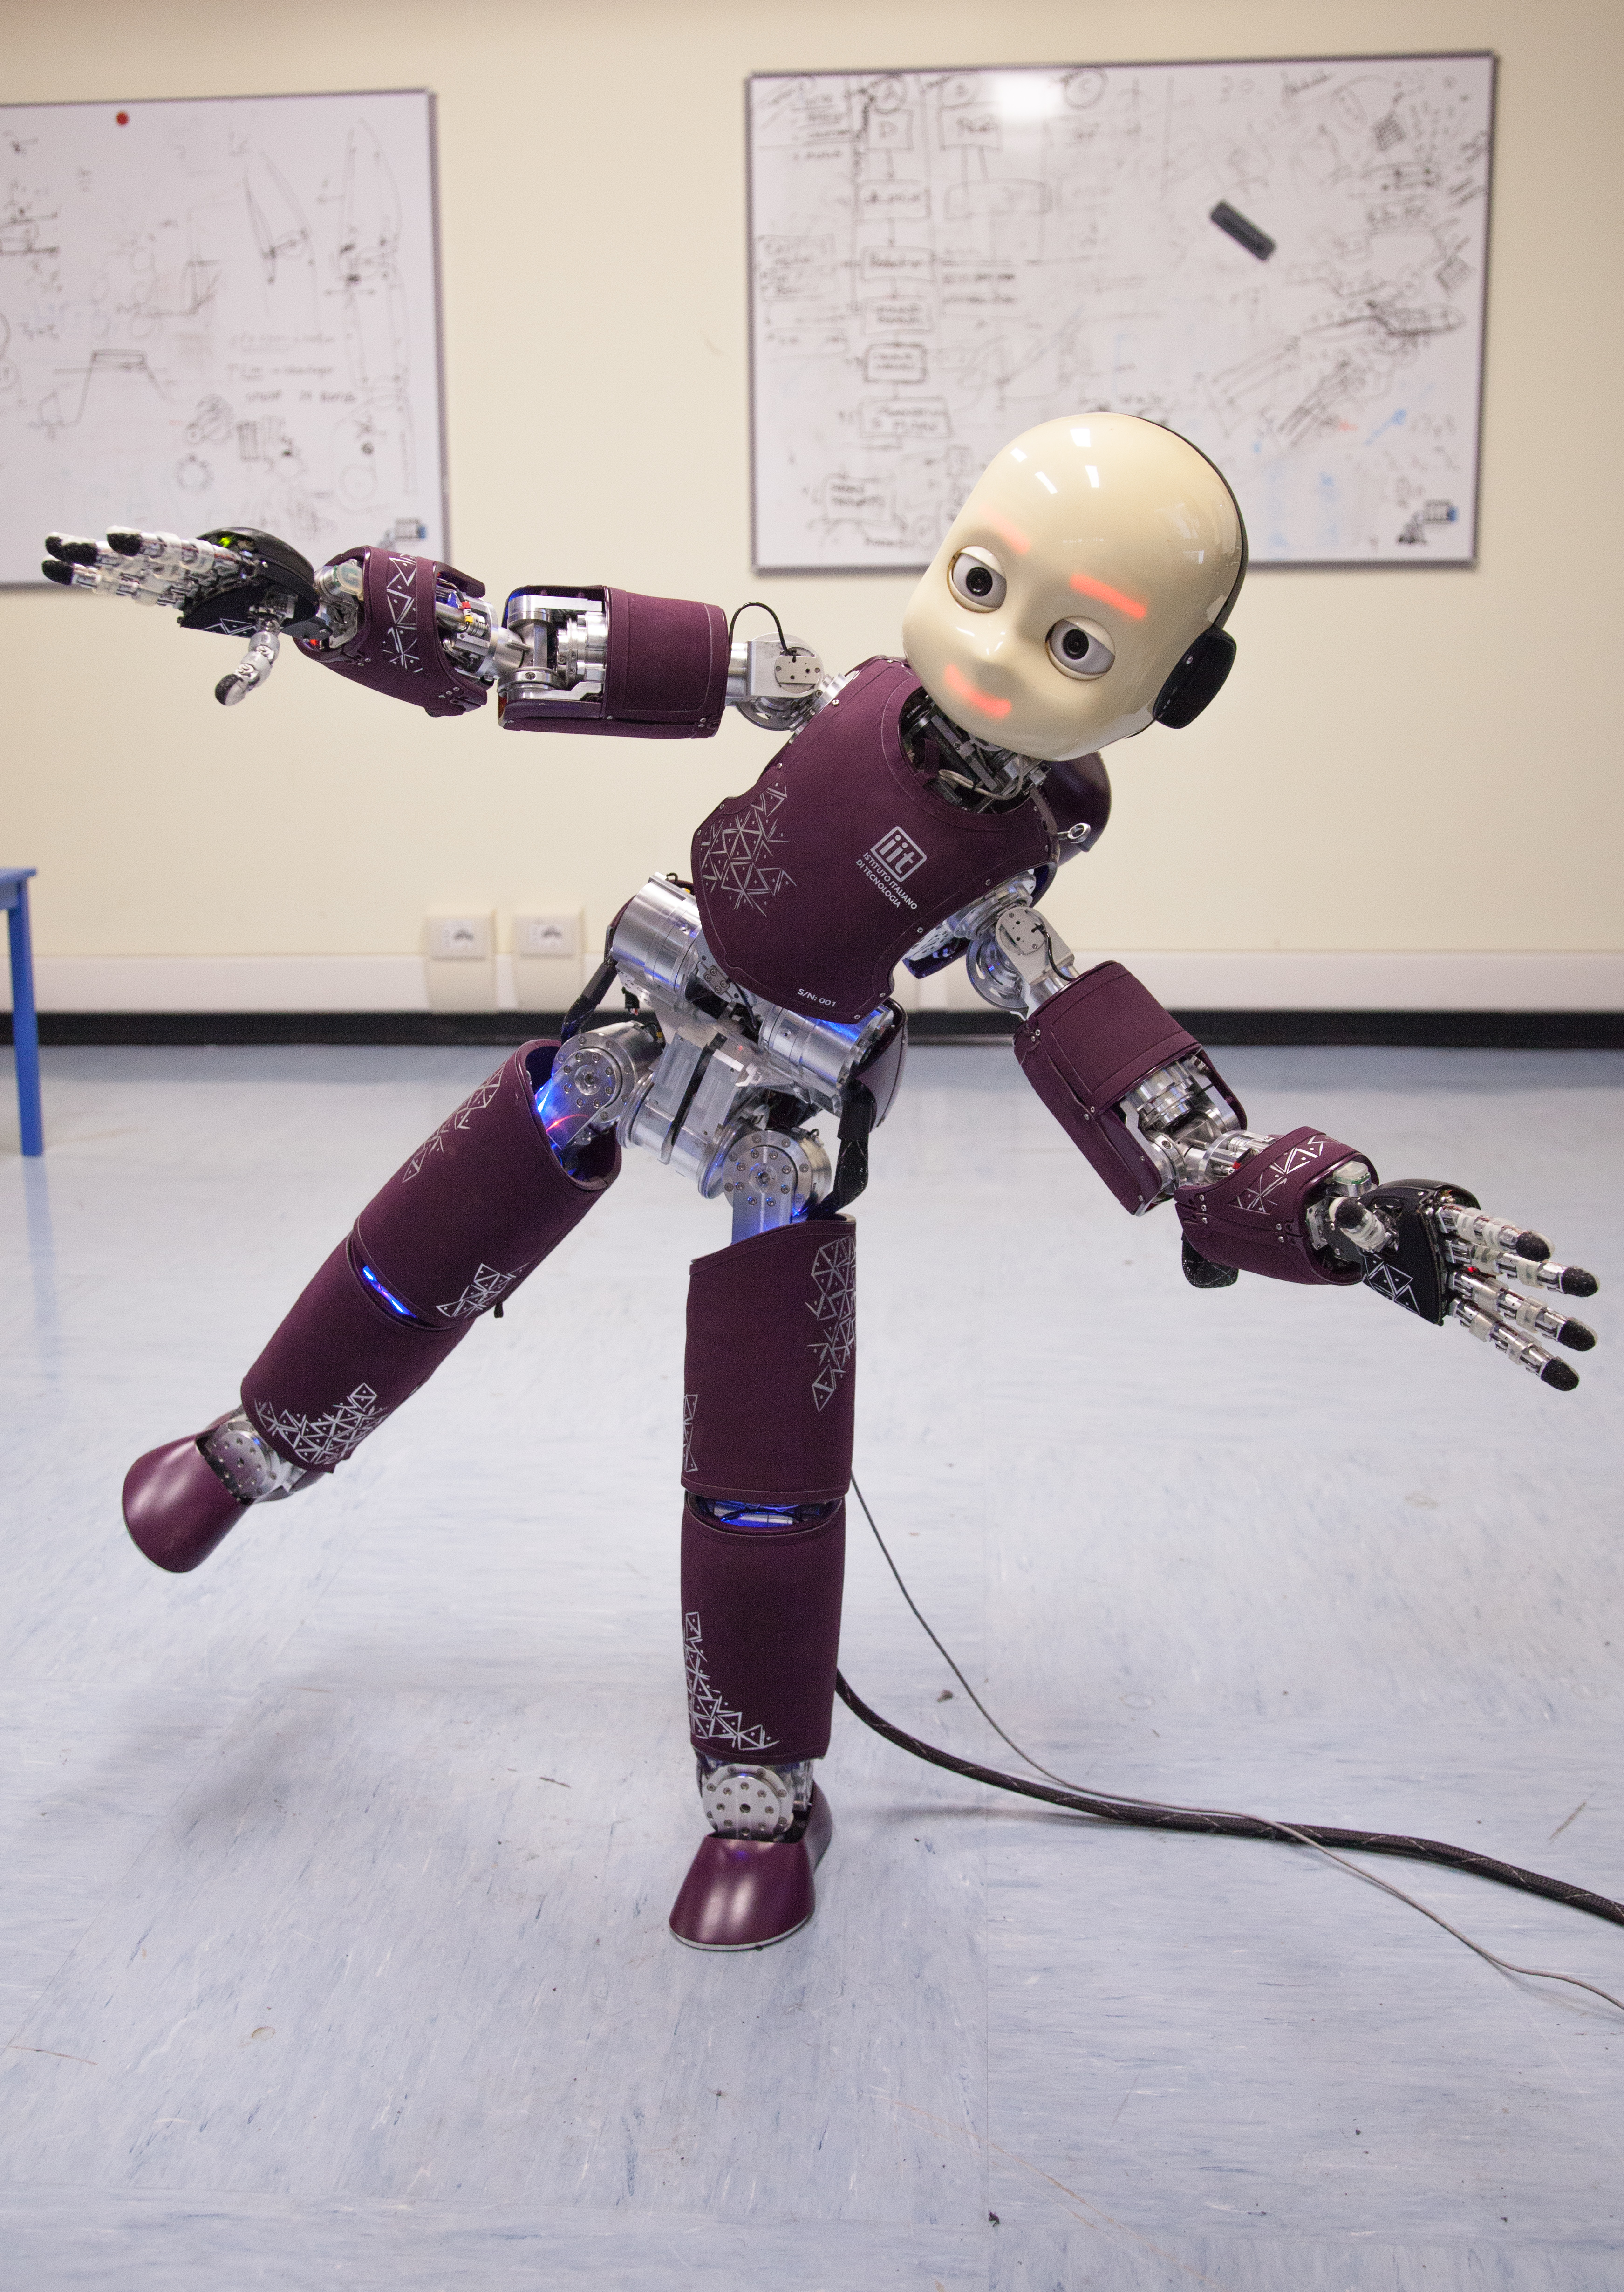
\includegraphics[width=0.7\textwidth]{icub-balancing.jpg}
\end{figure}

One of the research goals of the iCub project is 
to endow humanoids with advanced physical interaction capabilities. This is motivated by the idea that future robots will be required to physically interact with the environment and, in the long run, with humans. 
A key requirement for this \emph{interaction control} is the capability to measure and control the forces that a robot is exchanging with its environment, i.e. \emph{contact forces control}. While in traditional industrial applications this is achieved by by placing a six-axis force-torque sensor between the robot and the environment, this is not feasible in humanoid robotics, in which the contact location is typically not known a-priori. To overcome this limitations, a \emph{unique} set of dynamics-related sensors have been added during the years to the iCub. 

\begin{figure}[H]
\centering
\includegraphics[width=0.5\textwidth]{icub-ftsens.png}
\caption{Distribution of the six embedded six-axis force-torque sensors (green) available in iCub 2.5 .}
\label{fig:icub-ftsens}
\end{figure}

The main force sensors available on the iCub are six \emph{internal} six-axis force-torque sensors. Four of them are mounted at the base of each limb while two of them are mounted in feet right below the ankles. The locations of these sensors are highlighted in Figure~\ref{fig:icub-ftsens}. The placement of these sensors was dictated by practical reasons, as the hand structure would have not been not able to support a force-torque sensor mounted in it, but also to enable estimation of internal joint torques and external force-torque, as described in \citep{fumagalli2010learning} for a single limb and in Chapter~\ref{chap:extForceAndJntTorqueEstimation} of this thesis for the whole-body case.

\begin{figure}[h]

\centering
\includegraphics[width=1.0\textwidth]{icub-skin.png}
\caption{Distribution of the tactile sensors on iCub 2.5.}
\label{fig:icub-skin}
\end{figure}

While internal force-torque sensors are able to measure force-torque due to a combination of internal dynamics and of contact wrenches, they are in general unable to measure the location of a contact force, or its distribution over a contact surface. For addressing these concerns the iCub body has been covered with a distributed set of capacitive  elements  acting  as  tactile  sensors~\citep{maiolino2013}. The  entire  sensor  network  acts 
as an ``artificial skin'', constituted by a sandwich of different
flexible fabrics mounted on top of a flexible Printed Circuit
Board (PCB), so that the entire structure can be conformed
on surfaces of different curvatures. The majority of iCub 2.5 external surface has been covered by this ``skin'', as shown by Figure~\ref{fig:icub-skin}. 

\begin{figure}[H]
\centering
  \includegraphics[width=.4\linewidth]{icub-ems.png}
  \includegraphics[width=.4\linewidth]{icub-mtb.png}
\caption{Distribution of the inertial sensors i.e. gyroscopes (left) and accelerometers (right) in iCub 2.5~.}
\label{fig:distributedInertialSensing}
\end{figure}

To read the distributed tactile sensors, the iCub has been equipped with distributed network of dedicated electronic boards. Remarkably, this boards are equipped with a 3 Degree-of-Freedom (DOFs) accelerometer. Similarly, several motor control boards are distributed in the robot structure, and each motor control board is equipped with both a 3 DOFs accelerometer and a 3 DOFs gyroscops. Furthermore, an full-fledged Inertial Measurement Unit, equipped with a 3 DOFs magnetometer, accelerometer and gyroscope is mounted on the head of the robot. 
These arrangements, shown in Figure~\ref{fig:distributedInertialSensing} provides the iCub with a vast amount of distributed \emph{inertial} sensing, that has been exploited for fine calibration \citep{guedelha2016}.


These sensors form the basis for the use of the estimation and identification algorithms presented in the thesis, that are essential technologies to enable \emph{interaction force control}. To describe the presented algorithms, we need to provide a solid background in multibody dynamics, that will be also presented in the thesis. 

\section{Thesis Organization}
The following is a brief summary of the organization of the thesis. At the beginning of each chapter a discussion of the contribution with respect to the state of art of the specific chapter is given. 

\subsection{Modelling}
This thesis includes in the Chapters~\ref{chap:rigid-body}, \ref{chap:multibody} a self-contained derivation of the multi body dynamics and in Appendix~\ref{liegroups} its connection with Lie Groups theory. Particular focus is placed on the role of the \emph{base link} in free-floating dynamics, and in the different representation of \emph{base}-related quantities that are used in literature. This chapters form the theoretical basis for the rest of the thesis, devoted to \emph{estimation} and \emph{identification} of humanoid robot dynamics. 

\subsection{Estimation}
Chapter~\ref{chap:extForceAndJntTorqueEstimation} describes the algorithms used for the estimation of external forces and internal joint torques using internal six-axis force-torque sensors, distributed inertial sensing and a distributed tactile system, that are the set of sensors available on the iCub robot, as discussed in Section~\ref{sec:icub}. This 
part is mainly a generalization of already existing results \citep{fuma2010,ivaldi2011,Fumagalli2012,DelPrete2012} to the whole-body case.

\subsection{Identification}
The main contribution of Chapter~\ref{chap:ft-calib} are two new algorithms for calibration of six-axis force-torque sensors that can be performed \emph{in situ}, i.e., without removing the sensor from the hosting  system. These algorithms exploit the specific geometric of the gravity force-torque when expressed in the sensor frame. 

Chapter~\ref{ch:inertialParameters} introduces the concept of the identification of the inertial parameters of a single rigid body.
The main contribution of  this chapter is the definition of a new condition, the \emph{fully physical consistency} for a set of inertial parameters to determine if they can be generated by a physical rigid body. The proposed condition ensure both the positive definiteness and the triangular inequality of 3D inertia matrices as opposed to existing techniques in which the triangular inequality constraint is ignored.

Chapter~\ref{ch:inertialParametersMultiBody} generalize the identification problem to the case of a system compose by multiple rigid bodies, with particualr attention of the relations between the identifiability subspaces of the regressor associated with the different set of sensors. 
The main contribution of this chapter is the adaptation of the existing techniques for inertial parameters identification on humanoids to the specific set of sensors that is available on the iCub robot. While most existing techniques \citep{ayusawa2013,ogawa2014,Mistry2009} assume that either the contact forces or the joint torques measurement are available, in the iCub we only have a distributed tacticle system and a internal six-axis force-torque sensors. We propose a way of using internal six-axis force-torque sensor for estimation, and furthermore we demonstrate that the set of inertial parameters that are identifiable from the internal six-axis force-torque sensors are a superset of the one that we need to run the estimation algorithms presented in Chapter~\ref{chap:extForceAndJntTorqueEstimation}. 

\section{Technological Outcome}
The modelling formalism and the estimation algorithms presented in this thesis enabled the development of an whole-body controller on the iCub robot, that has been used to showcase highly dynamical balancing~\citep{pucci2016video} and has even permitted to the iCub to take part to an Italian Talent show as a participant~\citep{gotstalent}. 
The interested reader is referred to \citep{nori2015} for an integration paper describing the overall whole-body control architecture.

Furthermore, all the algorithms described in this thesis have been implemented in the open source C++ library iDynTree~\citep{idyntree}. The iDynTree is complete with documentation for installing it and using it. Furthermore, the library is equipped with bindings with MATLAB, Octave, Python, Lua and Java to enable its use in a wide set of platforms, fulfilling all the disparate needs that may arise in a research environment.  

